\chapter{More Searches}
We explore purely \textbf{local searches}  in the state space, evaluating and modifying one or more current states rather than  exploring paths from an initial state. 


\section{Local Search}
In some problems, path to goal is irrelevant and only the final configuration matters (eg. place 8 queens such that they don't attack each other).

\textbf{Local search} algorithms operate using a single current node and move only to neighbors of that node. Paths are not retained. Two advantages, 
\begin{itemize}
    \item Use little memory
    \item Can find reasonable solutions in large or infinite (continuous) state spaces. 
\end{itemize}
Local search is useful for solving pure \textbf{optimization problems}  in which aim is to find the best state according to an \textbf{objective function}.

We can consider the \textbf{state-space landscape}. It has a location (the state) and elevation (value of objective function or heuristic). If elevation is heuristic want to find the lowest valley - a \textbf{global minimum}, if its an objective function we want to find the highest peak - a \textbf{global maximum}. A \textbf{complete}  local search algo always finds a goal, an \textbf{optimal} one always finds a global max/min.

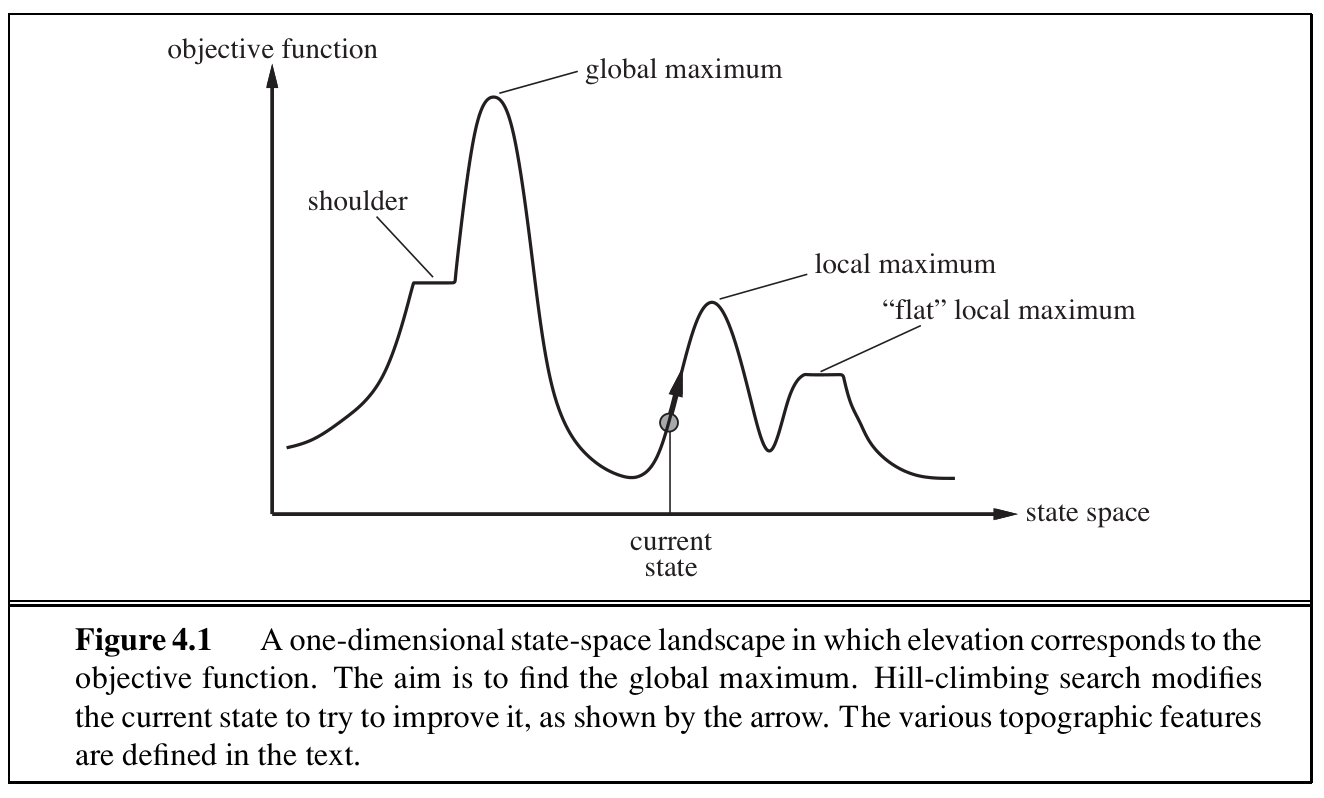
\includegraphics[width=\textwidth]{state_space_landscape}


\subsection*{Hill-climbing search}
A loop that continually moves in the direction of increasing value - uphill. Terminates when there is no neighbor with higher value. Does not maintain a search tree, data structure only maintains current node and value of objective function. Does not look ahead beyond immediate neighbors.

\begin{eg}
    In the \textbf{8-queens problem} we start with all 8 queens on the board. Successor of a state are all possible states by moving a single queen to another square in the same column (each state has $8 \times 7 = 56 $ successors). Heuristic $h$ is num of pairs of queens that are attacking each other. Global minimum is when no queen are attacking each other so when $h =  0$
\end{eg}

Sometimes called \textbf{greedy local search}  as it grabs a good neighbor without thinking anything ahead.


\begin{enumerate}
    \item Local maxima: A peak that is higher than each of its neighbors but lower than global minimum. Hill-climbing algos will reach here but will be stuck here as all its neighbors are worse than its current position.
    \item Ridges: Result in a sequence of local maxima that is difficult to navigate.
    \item Plateaux: A flat area of the state-space landscape. No uphill from which progress is possible. Algo might get lost.
\end{enumerate}

In each case algo can't make any more progress. For the 8 queen problem, hill-climbing algos get stuck 86\% of the time.

There are other variants such as \textbf{stochastic hill climbing} - chooses at random from the uphill moves: probability can vary with the steepness. Converges slowly but sometimes finds better solutions. \textbf{First choice hill climbing}  uses stochastic hill climbing by generating successors randomly until one is generated that is better than the current state. All these algos are incomplete (as we saw with the 8 queen problem).

\textbf{Random-restart hill climbing} randomly restarts to another initial state space if the default gets stuck. Is able to solve the 8 queens problem.


\subsection{Simulated annealing}
A hill-climbing algo that never makes a downhill move toward states with lower value is guaranteed to be incomplete (as it can get stuck at a local maxima or minima). A pure random walk for instance is complete but inefficient. A solution might be \textbf{combining} hill climbing and random walk so its both efficient and complete.

We switch pov from maximizing to minimizing (gradient descent). Analogy is pingpong ball on a bumpy surface. Letting the ball roll, it will stop at a local minima. If stuck we can shake the surface and hopefully bounce the ball out of there. So \textbf{simulated annealing} is shaking hard and then gradually reducing the intensity of the shaking.

So instead of picking the best move (like in hill climbing) it picks a \textbf{random move}. If the move improves the situation it is accepted, else the algo accepts the move with some probability less than 1 (decreases exponentially with how bad the move is). Probability also decreases as the temperature goes down. (If T goes down slowly, probability of finding global optimum approaches 1).


\subsection{Local beam search}
Initialized with $k$ random states rather than just one in memory. At each step, all successors of all $k$ searches are generated. If any one finds goal, algorithm halts. Else it selects $k$ best successors from the complete list and repeats. \textbf{Not} the same as $k$ random restarts in parallel. In local beam search useful information is \textbf{passed among the parallel search}. For instance if the $k$th search is stuck and the  $k-1$ search finds two good successors, the $k$th search with move to one of the two.

Can cause a lack of diversity where they converge to being concentrated in a small region making it a little more than an expensive hill climbing. \textbf{Stochastic beam search} is a variant - chooses $k$ successors at random (instead of the best) probability of choosing is a function of its value.


\subsection{Genetic algorithms}
Variant of stochastic beam search in which successor states are generated by combining two parent states than by modifying a single state.

So we start with $k$ random initial states (the population). To produce the next generation of states we have an objective function (in GA terms the \textbf{fitness function}). The function returns higher value for better states. For instance for the 8 queen problem we can construct a 8 digit string each number representing the position of the queen in that column. We can mate two strings by using the first half of the first and second half of the second (we decide which strings to mate using their fitness function). 

Crossover often takes \textbf{long steps}  early in and short steps \textbf{later on}.






